\chapter{Teaching}
\label{lehre}
\section{General}

The "'Teaching"' section contains the most important links for your daily teaching.
Here you can view information about the courses, the teaching schedule, attendance lists, and semester schedules.

\section{Courses}
\label{lehre_lehrveranstaltungen}

On the "'Courses"' page you can first select the degree program and the semester you wish to view.

\begin{figure}
	\centering
	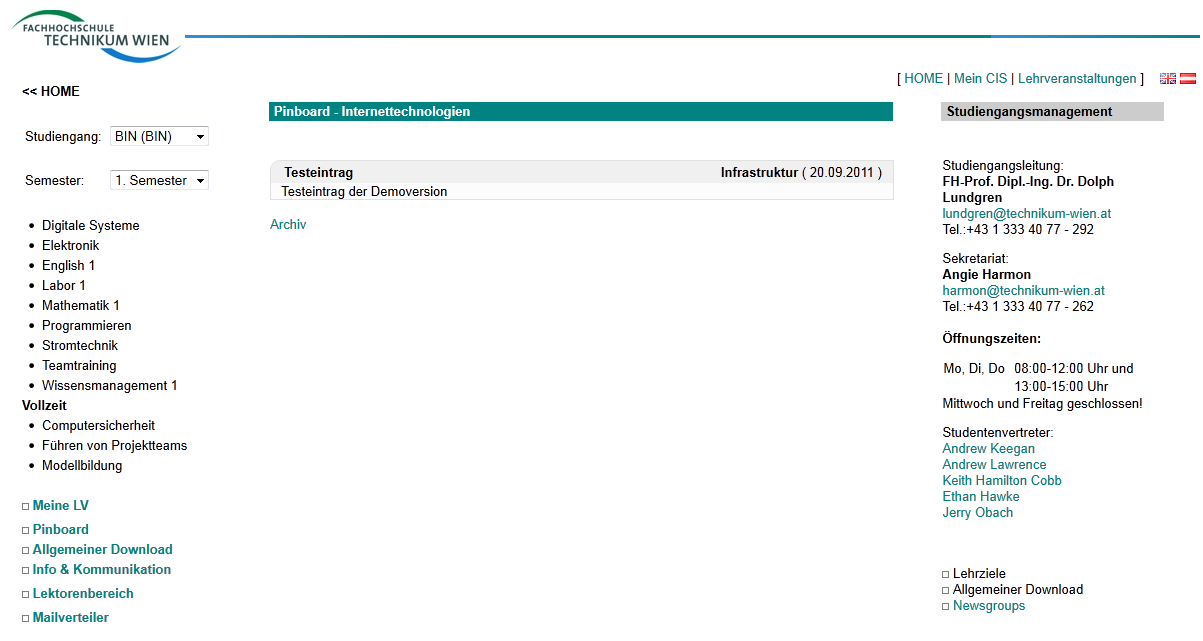
\includegraphics[width=0.70\textwidth]{CIS_Lehrveranstaltungen.png}
	\caption{CIS Courses}
	\label{CIS_lehrveranstaltungen}
\end{figure}

The news in the main window consists of the general news and specific news for the chosen degree program. If no specific news is available, only the general news entries will be displayed.

After selecting the desired degree program, all the active courses are listed.
If you select one of the courses, an overview will appear in the main window with all the tools and information available for this course. (see Fig. \ref{CIS_lehrveranstaltungen})

\begin{figure}
	\centering
	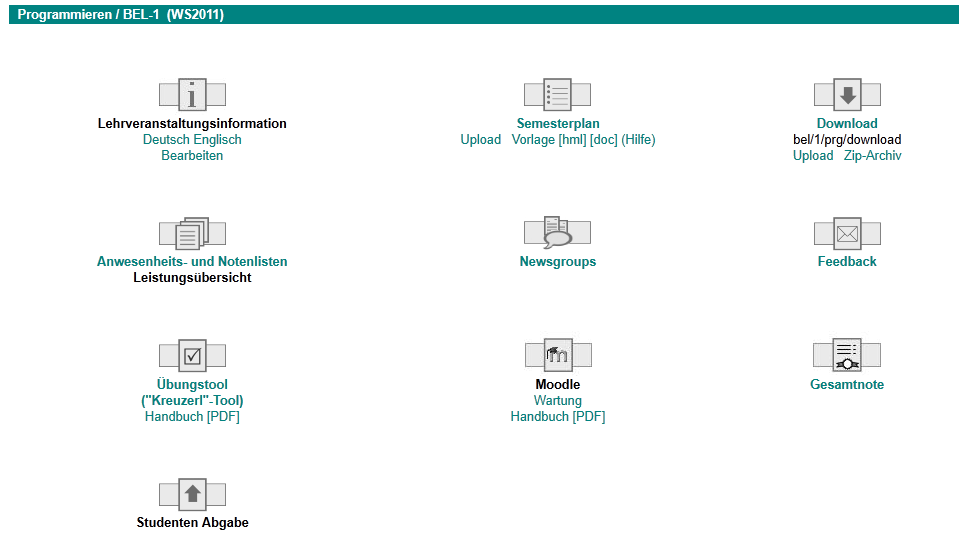
\includegraphics[width=0.70\textwidth]{CIS_Lehrveranstaltungen_Icons.png}
	\caption{CIS Courses Details}
	\label{CIS_lehrveranstaltungen}
\end{figure}

Here you can view the course information, semester plan, or the download area as well as generate attendance lists.
Furthermore, 3 tools are available to help you in your teaching: The activity tool, the student upload tool and the e-learning platform Moodle.

In the menu on the left you will also find the following sections:
\begin{description}
	\item [My Courses:] These are the courses in which you personally are a teacher or student.
	\item [Pinboard:] The news view with current information.
	\item [Global Download:] A link to the download area for the degree program.
	\item [Info \& Communication:] Here you will find a link to the teaching schedule, as well as to the webmail for you to manage your email.
	\item [Lecturer's Section:] Here you can edit the course information, upload documents and publish news entries if you possess the required user rights.
	\item [Mailing List:] Here you will find an overview of all the mailing lists at the UAS TECHNIKUM WIEN. By default, students are not granted access to large mailing lists.
\end{description}

\section{Electives}
\label{lehre_freifaecher}

Students can choose from any of the electives offered. The teacher is responsible for arranging the course times and dates.
The electives page is very similar to the courses page with only minor differences.
Here too it is possible to enter course information and semester plans as well as print out attendance lists.

On the left you will find the menu item "'Enrollment"' where you can mark all the desired electives and enroll for them by clicking on the "'Save"' button.
You can view the current enrollment status in the "'overview"'.

Withdrawal from an elective course is currently only possible by contacting the administrative assistant directly.

\section{Teaching Schedule}
\label{lehre_lvplan}

The teaching schedule is the UAS TECHNIKUM WIEN timetable.
You can select your personal schedule, the room schedule, the teaching schedule or the teaching group schedule.

\begin{figure}
	\centering
	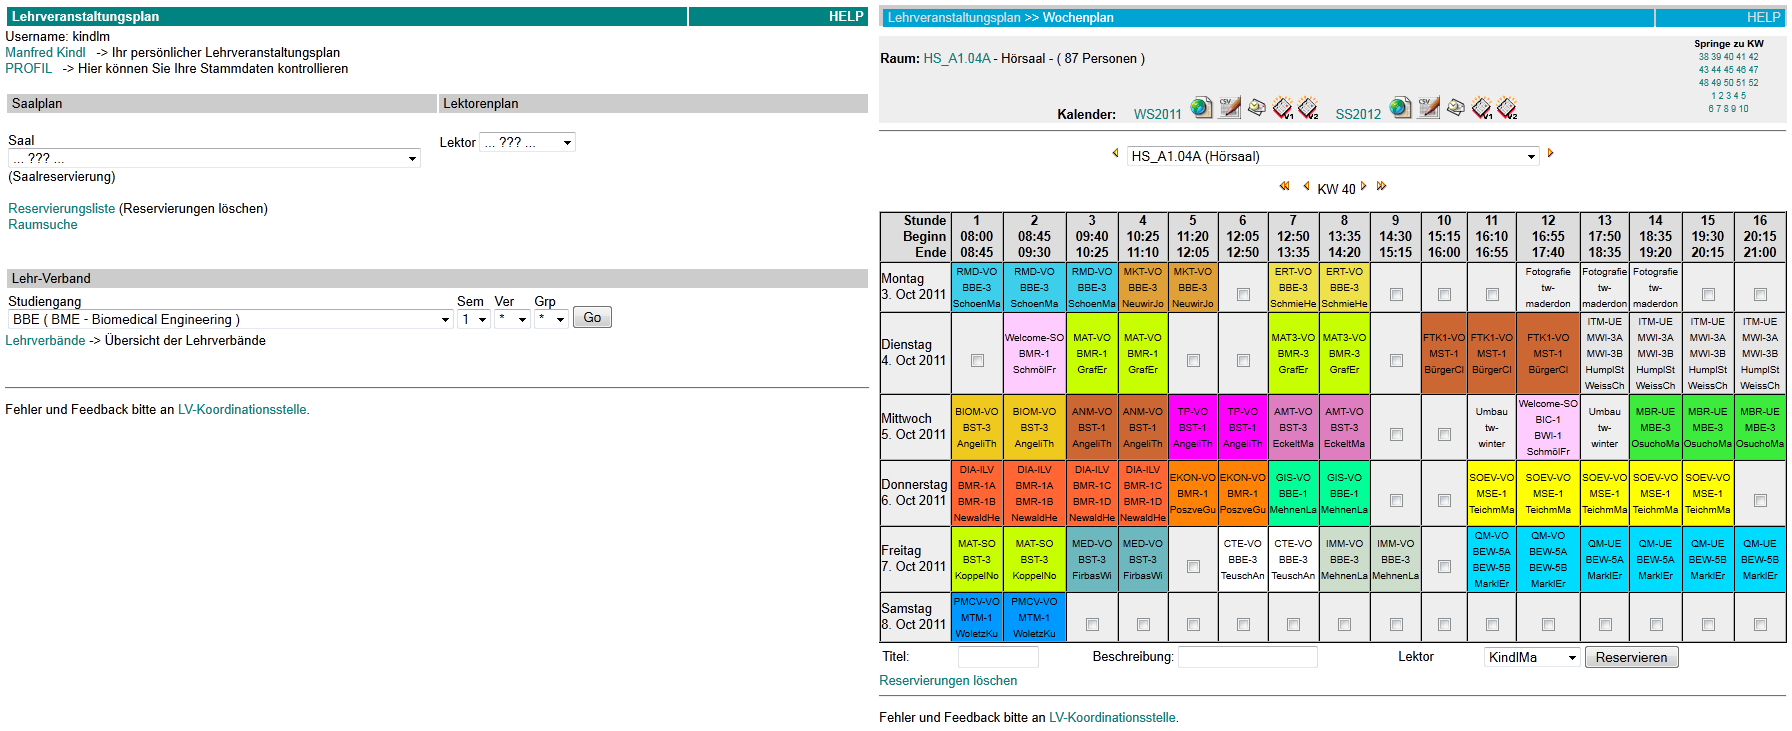
\includegraphics[width=1\textwidth]{CIS_Lvplan.png}
	\caption{CIS Teaching Schedule}
	\label{CIS_Teaching_Plan}
\end{figure}

\begin{description}
	\item [Personal Teaching Schedule:] Here you can view the teaching schedules that affect you personally. You only see the hours for your allocated group, any electives, if applicable, and your own reservations.
	\item [Room Schedule:] In this list you will find all the classrooms at the UAS TECHNIKUM WIEN and you can then view the schedule for each room. If you have the necessary rights, you can also make reservations using the room schedule.
	\item [Teaching Schedule:] allows you to view the timetable for a specific lecturer.
	\item [Teaching -Teaching Group:] Here you can view the schedule of each degree program optionally limited by semester, division and group.
\end{description}

\subsection{The Calendar View}

By clicking on the arrows here, you can move one week or four weeks forwards or backwards.
In the room schedule view you have an additional drop-down menu to scroll between the rooms.
If you click on an assigned unit, a details window will appear with additional information.

In addition, it is also possible to open the semester plan (overview with all the weeks arranged in a column) by clicking on WS20xx or SS20xx.

With the 5 icons next to each semester plan, you can export the teaching schedule to other clients (e.g. Outlook, Sunbird, Smartphone,...).

\subsection{Making Reservations}

You will require the appropriate rights (employees, lecturers, student representatives) to be able to reserve a room.
Select the location you want from the room schedule and mark the checkboxes for the units you want to reserve.
Afterwards, enter a title and a short description of the reason you wish to reserve the room.
Finally, click on the "'Reserve"' button.

\info{The reserved unit is visible only in the room schedule and in your personal schedule. If you want to make the reservation visible for a degree program, semester, or division, please contact the Scheduling Office}

\subsection{Deleting a Reservation}

You can view your reservations in the room schedule by clicking on "'Reservations List"' in the main menu or delete them by clicking on "'Delete Reservations"'.

\subsection{Room Information}

When you are in the room schedule, you can click the room name at the top left.
This will open a page where you can view detailed information about the equipment in the room, location information and pictures of the room.

\section{Documents}

Here you will find important and helpful documents related to everyday university life. Depending on your rights, you can access various folders and download files.

\section{Software for Teaching}

Here you will find software that can be used to help you in your teaching.

\begin{description}
	\item [Softgrid:] Is an environment-independent virtualization software with the application no longer being installed on the end device, but provided as a central application available any time. The local caching of the required applications allows you to take these applications "'with you"' and use them offline for up to 40 days. For installation details, see the "'Infrastructure"' section.
	\item [Dynamic Power Trainer:] Is a professional authoring software that you can use to create eLearning courses.
	\item [Moodle:] Is an object-oriented course management system and an open-source learning platform. The software offers possibilities for supporting collaborative teaching and learning methods.
\end{description}

\section{Plagiarism Check}

Both students and lecturers can submit their scientific work here for a plagiarism assessment by the external platform "'Ephorus"'.